\documentclass[a4paper,11pt]{article}
% Use ctrl + alt + V to view live pdf

% Packages
\usepackage[utf8]{inputenc} % For encoding
\usepackage[T1]{fontenc} % Better handling of accented characters and hyphenation
\usepackage{microtype} % Improves spacing and justification
\usepackage{amsmath, amssymb} % For equations and symbols
\usepackage{graphicx} % For including graphics/images
\usepackage{caption} % For customizing figure and table captions
\usepackage{subcaption} % For subfigures and subcaptions
\usepackage{float} % For fixing figure and table positions
\usepackage{booktabs} % For professional-looking tables
\usepackage{siunitx} % For consistent typesetting of units and numbers
\usepackage[margin=2cm]{geometry} % Adjusts page margins
\usepackage{fancyhdr} % For custom headers and footers
\usepackage{lmodern} % For a professional-looking font (main body font)
\usepackage{titlesec} % For title customization
\usepackage{array} % For custom table formatting
\usepackage[colorlinks=true, linkcolor=black, urlcolor=black]{hyperref} % Colored links without boxes
\usepackage{cleveref} % For improved cross-referencing    
\usepackage{multirow}
\usepackage{enumitem}
\usepackage{listings}
\usepackage{xcolor}
\usepackage{textcomp}
\usepackage{tabularx}
\usepackage{changepage}
\usepackage{tikz}
\usepackage{pdfpages}
\usepackage[table]{xcolor}
\usetikzlibrary{shapes.geometric, arrows}
% --- C++ Style ---
\lstdefinestyle{cpp-style}{
    language=C++,
    basicstyle=\ttfamily\footnotesize,
    keywordstyle=\color{blue}\bfseries,
    stringstyle=\color{orange},
    commentstyle=\color{gray}\itshape,
    numbers=left,
    numberstyle=\tiny\color{gray},
    numbersep=10pt,
    backgroundcolor=\color{white},
    showspaces=false,
    showstringspaces=false,
    breaklines=true,
    breakatwhitespace=true,
    tabsize=4,
    captionpos=b,
    frame=single,
    rulecolor=\color{black},
}

% --- Python Style ---
\lstdefinestyle{python-style}{
    language=Python,
    basicstyle=\ttfamily\footnotesize,
    keywordstyle=\color{blue}\bfseries,
    commentstyle=\color{gray}\itshape,
    stringstyle=\color{green!50!black},
    frame=single,
    breaklines=true,
    showstringspaces=false,
    captionpos=b
}
\renewcommand{\lstlistingname}{Code}
% Custom settings
\pagestyle{fancy}
\fancyhf{}
\fancyhead[L]{\textit{SF4 - DataLogger}} % Header left
\fancyhead[R]{\textit{Will Hewes - wh365}} % Header right 
\fancyfoot[C]{\thepage} % Footer center
\setlength{\headheight}{15pt} % Header height
\setlength{\parindent}{0em} % Indentation for paragraphs
\setlength{\parskip}{0.5em} % Add spacing between paragraphs
\setlength{\abovedisplayskip}{1em}
\setlength{\belowdisplayskip}{1em}
\setlength{\abovedisplayshortskip}{1em}
\setlength{\belowdisplayshortskip}{1em}
% \setlist{topsep=0.2em, partopsep=0em, itemsep=0.1em, parsep=0em}

\graphicspath{{Images/}}

% \renewcommand{\arraystretch}{1.2}

% Title formatting
\renewcommand{\maketitle}{
    \begin{center}
        \LARGE \textbf{ENGINEERING TRIPOS PART IIA} \\[0.5em]
        \Large \textbf{SF4 - DataLogger} \\[0.5em]
        \textbf{Final Report} \\[1.5em]
        \vspace{-1em}
        \small Will Hewes - wh365 \\ 
        Pembroke College \\ 
        \vspace{0.5em}
    \end{center}
}

\begin{document}
\pagenumbering{gobble}
% 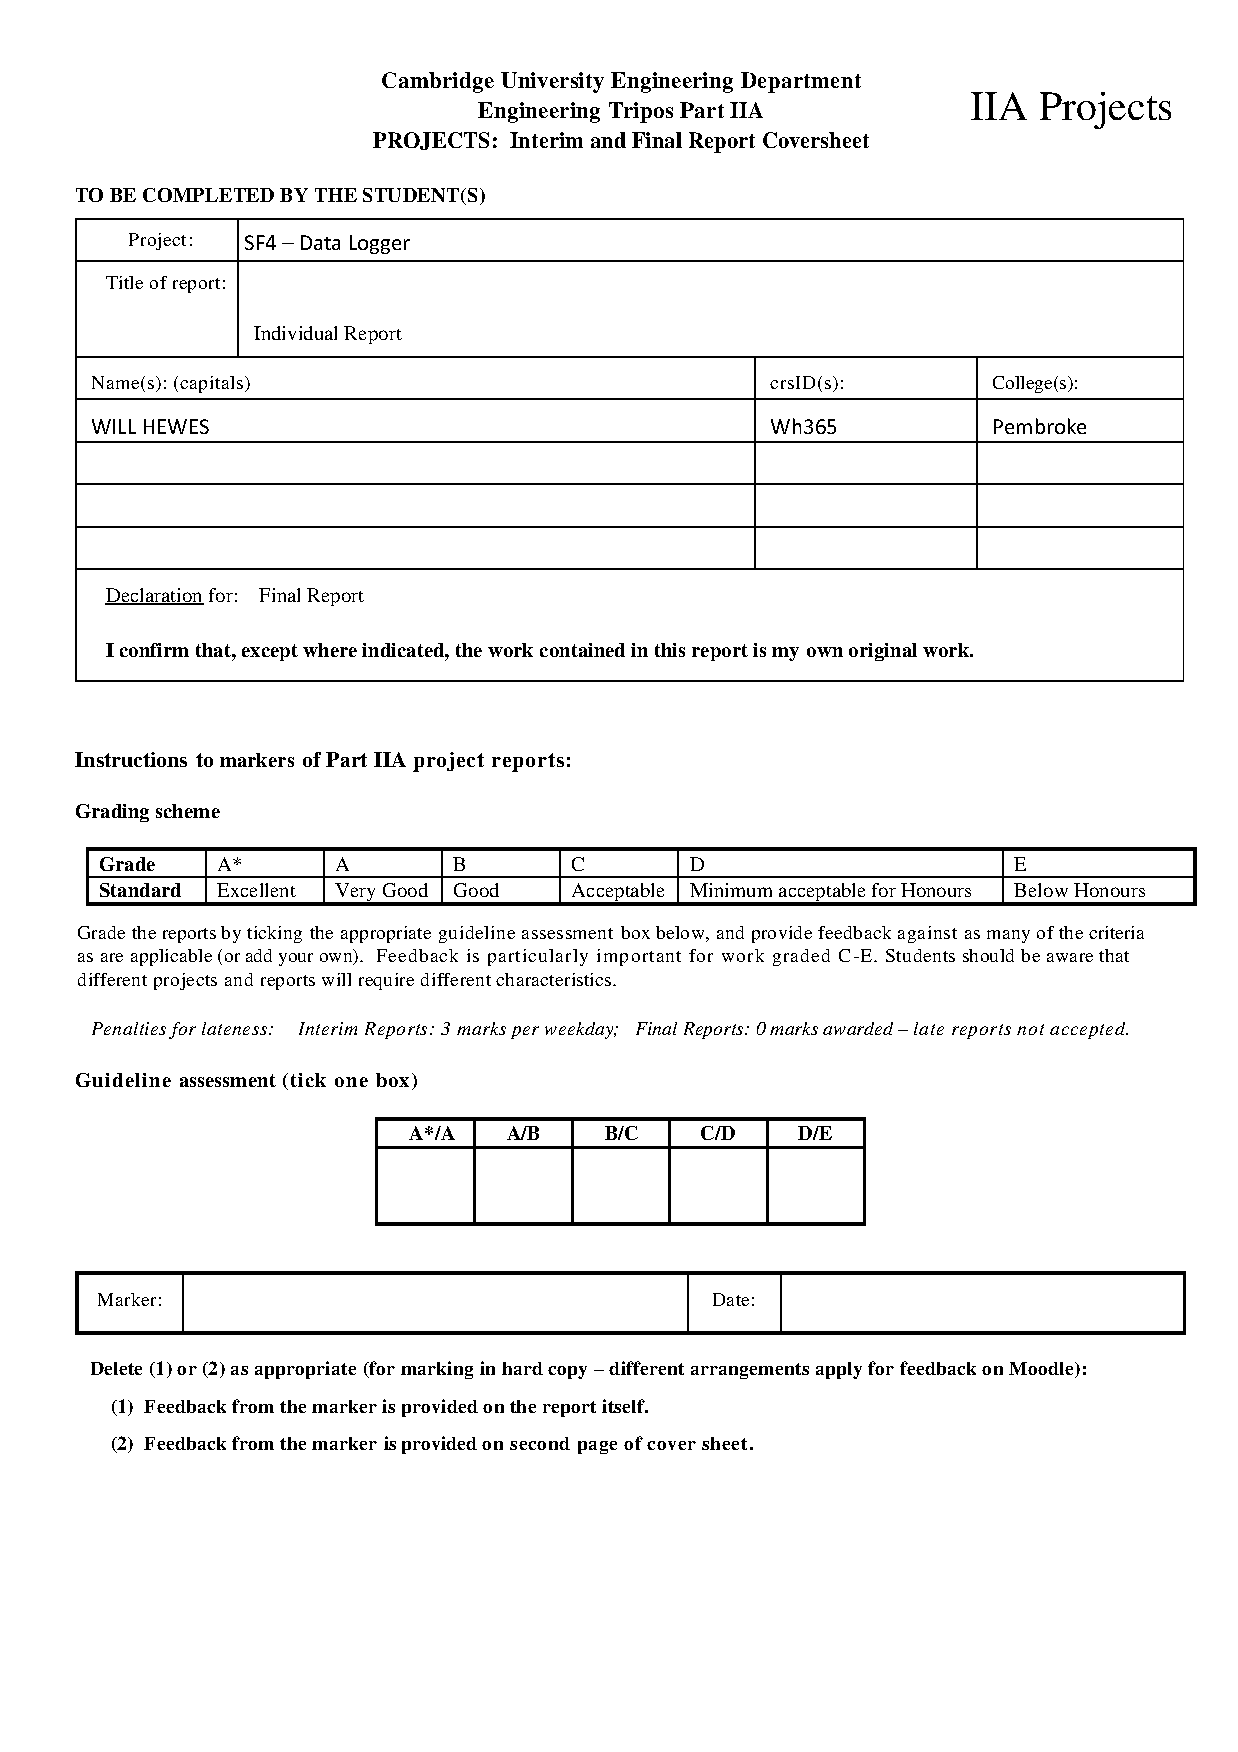
\includepdf[pages=-]{Handouts/IIA_Project_Coversheet Final Report.pdf}
\maketitle
\hrule
\tableofcontents
\newpage
\pagenumbering{arabic} \setcounter{page}{1}

\section{Introduction}
\label{sec:introduction}

\section{System Summary}
\label{sec:summary}

\section{Project Management}
\label{sec:project_management}

\section{System Architecture}
\label{sec:architecture}
\subsection{Block Diagram}
\label{sec:block_diagram}
\subsection{Circuit Design}
\label{sec:circuit_design}
\subsection{Watering Mechanism}
\label{sec:water_system}

\section{Initial Development}
\label{sec:initial_development}
\subsection{Sensor Prototyping}
\label{sec:sensor_prototyping}
\subsection{GUI}
\label{sec:gui_simulation}
\subsection{Communication Protocol}
\label{sec:comm_protocol}

\section{Final Implementation}
\label{sec:final_implementation}
\subsection{Firmware}
\label{sec:firmware}
\subsubsection{Main Loop}
\label{subsec:main_loop}
\subsubsection{Signal Processing}
\label{subsec:firmware_processing}
\subsection{Software}
\label{sec:software}
\subsubsection{Module Structure}
\label{subsec:software_modules}
\subsubsection{User Interface}
\label{subsec:software_ui}

\section{Technical Challenges}
\label{sec:technical_problems}

\section{Further Improvements}
\label{sec:further_improvements}

\section{Conclusion}
\label{sec:conclusion}


\newpage
\appendix
\begin{thebibliography}{9}

\bibitem{arduino_servo}
Arduino. \textit{Servo Motor Basics with Arduino} : \\
\url{https://docs.arduino.cc/learn/electronics/servo-motors/}

\bibitem{tmp36}
Analog Devices. \textit{TMP35/TMP36/TMP37 Data Sheet} : \\
\url{https://www.analog.com/en/products/tmp36.html} 

\bibitem{arduino_tmp36}
ArduinoGetStarted. \textit{Arduino - TMP36 Temperature Sensor} : \\
\url{https://arduinogetstarted.com/tutorials/arduino-tmp36-temperature-sensor}

\bibitem{dfrobot}
DFRobot. \textit{Capacitive Soil Moisture Sensor SKU SEN0193} : \\
\url{https://wiki.dfrobot.com/Capacitive_Soil_Moisture_Sensor_SKU_SEN0193}

\bibitem{pinch_valve_design}
Printables. \textit{Pinch Valve Powered by Servo} : \\
\url{https://www.printables.com/model/247744-pinch-valve-powered-by-servo/files}

\end{thebibliography}

\section{Interim Report}
% 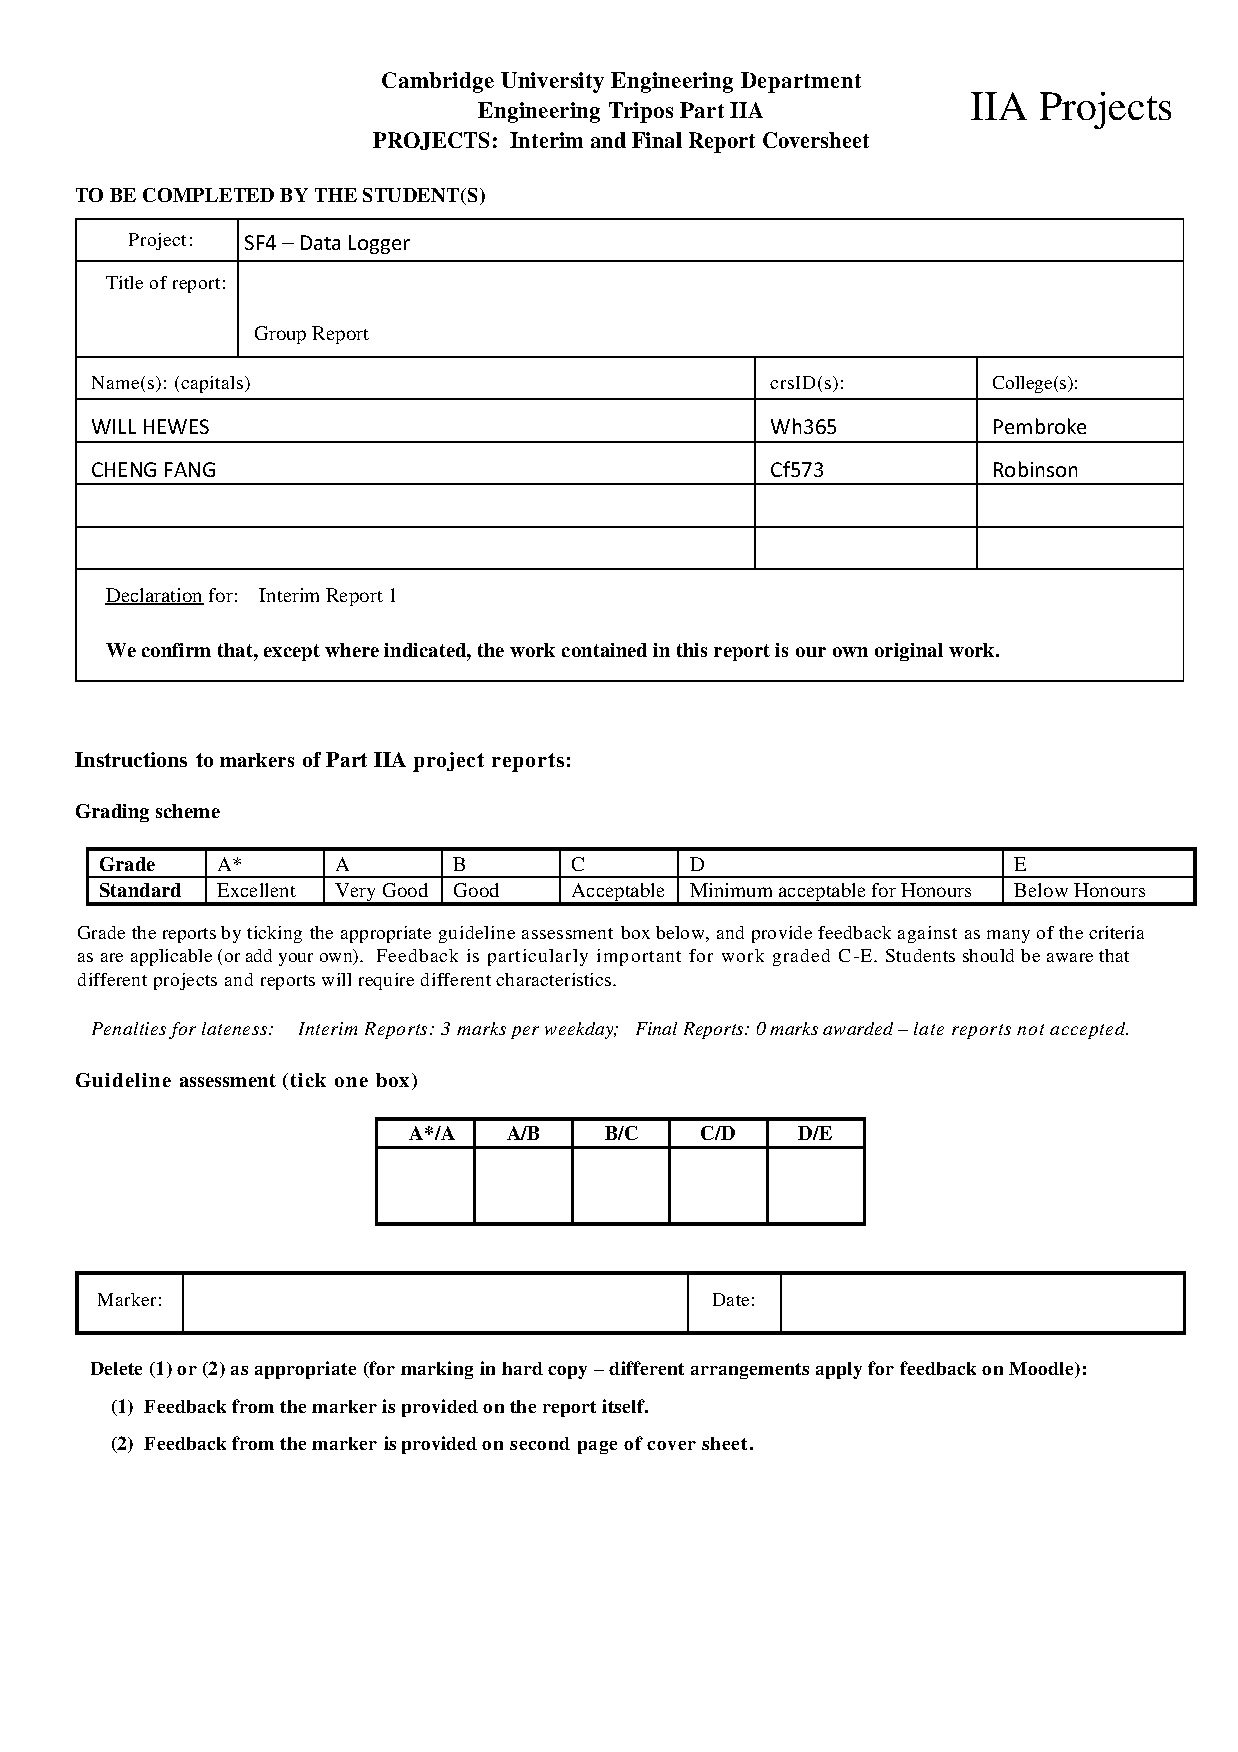
\includepdf[pages=-]{Reports/First Interim Report.pdf} % e.g. [pages={1,3-5,7}] to include pages 1,3,4,5,7
% Featuring the Interim Report

\end{document}